\documentclass[border=10pt]{standalone}

\usepackage{pgfplots}
\pgfplotsset{compat=1.18}
\usepgfplotslibrary{fillbetween}

\begin{document}

% \begin{tikzpicture}
%     \begin{axis}[ymin = -0.1, ymax = 1.1]
%         \addplot[name path = parab, domain = -1:1] {x^2};
%         \addplot[name path = floor, draw = none] coordinates {(-1,-0.1) (1,-0.1)};
%         \addplot[color=gray] fill between[of = parab and floor];
%     \end{axis}
% \end{tikzpicture}

% \begin{tikzpicture}
%     \begin{axis}[ymin = -0.1, ymax = 1.1]
%         \addplot[name path = parab, domain = -1:1] {x^2};
%         \addplot[name path = floor, draw = none] coordinates {(-1,-0.1) (1,-0.1)};
%         \addplot[color=gray] fill between[of = parab and floor, soft clip = {domain = -0.5:0.5}];
%     \end{axis}
% \end{tikzpicture}

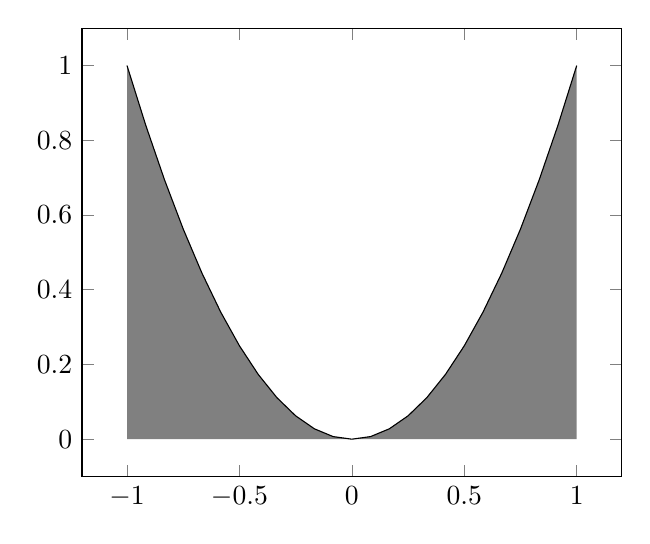
\begin{tikzpicture}
    \begin{axis}
        \addplot[name path = parab, domain = -1:1] {x^2};
        \addplot[name path = floor, draw = none] coordinates {(-1,0) (1,0)};
        \addplot[color=gray] fill between[of = parab and floor];
    \end{axis}
\end{tikzpicture}

\end{document}